\documentclass[11pt,a4paper]{article}
\usepackage[a4paper,margin=2cm]{geometry}
\usepackage[T1]{fontenc}
\usepackage{lmodern}
\usepackage{microtype}
\usepackage{booktabs,tabularx,array}
\usepackage{enumitem}
\usepackage{xcolor}
\usepackage{tikz}
\usetikzlibrary{arrows.meta,positioning,fit,backgrounds,calc}
\usepackage[most]{tcolorbox}
\usepackage[hidelinks]{hyperref}
\usepackage{titlesec}
\usepackage{float}
\usepackage{caption}
\captionsetup{font=small,labelfont=bf,skip=3pt}

\definecolor{accent}{HTML}{1F4E79}
\definecolor{soft}{HTML}{EAF1F8}
\definecolor{toolc}{HTML}{FFF4E0}
\definecolor{safec}{HTML}{FDECEC}
\definecolor{okc}{HTML}{E8F5E9}
\definecolor{specc}{HTML}{F3E8FD}
\definecolor{greyc}{HTML}{F4F4F4}

\titleformat{\section}{\large\bfseries\color{accent}}{\thesection}{0.6em}{}
\titlespacing*{\section}{0pt}{7pt}{2pt}
\titleformat{\subsection}{\normalsize\bfseries}{\thesubsection}{0.5em}{}
\titlespacing*{\subsection}{0pt}{4pt}{1pt}
\setlist{nosep,leftmargin=1.2em}
\setlength{\parindent}{0pt}
\setlength{\parskip}{3pt}
\renewcommand{\arraystretch}{1.12}
\newcolumntype{L}{>{\raggedright\arraybackslash}X}

\newtcolorbox{keybox}[1][]{colback=soft,colframe=accent,boxrule=0.6pt,arc=2pt,
  left=5pt,right=5pt,top=3pt,bottom=3pt,fonttitle=\bfseries,#1}

\tikzset{
  box/.style={draw=accent,fill=soft,rounded corners=2pt,align=center,font=\small,inner sep=3pt,minimum height=8mm},
  tool/.style={draw=orange!70!black,fill=toolc,rounded corners=2pt,align=center,font=\footnotesize,inner sep=2.5pt,minimum height=7mm},
  ok/.style={draw=green!45!black,fill=okc,rounded corners=2pt,align=center,font=\footnotesize,inner sep=2.5pt,minimum height=7mm},
  bad/.style={draw=red!60!black,fill=safec,rounded corners=2pt,align=center,font=\footnotesize,inner sep=2.5pt,minimum height=7mm},
  spec/.style={draw=violet!70!black,fill=specc,rounded corners=2pt,align=center,font=\small,inner sep=3pt,minimum height=8mm},
  kb/.style={draw=black!55,fill=greyc,rounded corners=2pt,align=center,font=\footnotesize,inner sep=2.5pt,minimum height=7mm},
  arr/.style={-{Stealth[length=2.2mm]},thick,accent},
  darr/.style={-{Stealth[length=2mm]},dashed,thick,violet!70!black},
  garr/.style={-{Stealth[length=2mm]},black!55},
}

\begin{document}

%================ TITLE =================
\begin{center}
{\LARGE\bfseries\color{accent} CounselCopilot}\\[3pt]
{\Large\bfseries\color{accent} Catching Policy and Legal Conflicts in NDA Drafts with\\[1pt]
Applicability-Aware Retrieval and Verified Speculation}\\[6pt]
{\large LMA Group Project 2026 \,--\, Project Proposal}\\[3pt]
\textbf{Team members (roll numbers):}\\[1pt]
2025201049 \qquad 2025201044 \qquad 2025201068 \qquad 2025201038
\end{center}

\begin{keybox}[title=Summary in three lines]
\textbf{Problem:} legal consultants who draft NDAs change often and cannot learn hundreds of pages of company policy, so their drafts quietly \emph{miss} required terms or break rules.\\
\textbf{Idea:} a drafting copilot that finds every company rule and Indian-law provision that \emph{applies to this deal}, checks the draft against each one with exact tools, and cites both sides. While the consultant is still writing, it runs the review early and reuses the result only if the finished clause matches.\\
\textbf{Test:} on real NDAs with expert-labelled and planted defects, does this catch more omissions with fewer false alarms than standard RAG, long-context prompting and checking every rule, and does early review cut waiting time without changing the result?
\end{keybox}

%================ 1 =================
\section{Domain, target user and problem}
\textbf{Domain:} Legal. \textbf{Scope:} one contract type (NDAs), one jurisdiction (India), three companies' policy packs.\\
\textbf{Target user:} a legal consultant (contract staff, outsourced counsel or junior associate) drafting NDAs for a company, with a senior lawyer who signs off.

\textbf{Problem statement.}
Companies spread their NDA requirements across many documents: data-protection, IP and vendor policies, an approval matrix and past negotiated positions.
The consultants who draft NDAs rotate often, and a new consultant cannot absorb all of this in a few days.
Their typical mistake is not bad wording but a \emph{missing} or non-compliant term, such as no data-return clause, a confidentiality period shorter than policy allows, or a foreign governing law that needs General Counsel approval.
Some drafts also contain terms that are risky under Indian law, such as a broad non-compete, which is void as a restraint of trade under s.27 of the Indian Contract Act, 1872.
These misses surface later as disputes.
A reviewer that reads the draft once cannot find a missing clause, because there is nothing in the text to point at.
We want a copilot that checks every applicable rule, cites it, and acts as knowledge transfer at the moment the consultant needs it.

\textbf{Why it matters.} NDAs are the most frequently signed contracts, consultant turnover is high, and one missed rule can expose a company's data or IP. A senior lawyer can verify a cited flag in seconds but cannot re-read every policy for every draft.

%================ 2 =================
\section{What is missing in existing approaches}
\begin{itemize}
\item \textbf{Contract-error benchmarks} (CLAUSE, EACL Findings 2026; ContractScrub, 2026) test single prompted models on errors inside one contract; the best macro recall on ContractScrub is only 0.75. \textbf{ContractEval} (NLLP 2025) finds that open models wrongly answer ``no such clause'' in about 25--30\% of cases. None of them checks a draft against a \emph{company's own policies}.
\item \textbf{PolicyGuard} (arXiv 2606.32004, 2026), the closest work, compiles one company's NDA playbook into logic rules and checks every rule. It is evaluated on 5 confidential contracts that cannot be released, treats absence only through per-rule questions, and ignores deal-specific applicability.
\item \textbf{Industry tools} (Harvey, LegalOn, Spellbook) offer ``playbook review'' with private evaluations only. \textbf{There is no open benchmark for policy compliance of NDAs that tests omissions.}
\item \textbf{Speculative agents} (Speculative Actions, PASTE; Speculative Interaction Agents, 2026) start work early to hide latency. The last of these speculates on unfinished user speech but loses a little accuracy. None of them verifies reuse exactly or studies document drafting.
\end{itemize}

%================ 3 =================
\section{Research questions and hypotheses}
\begin{keybox}
\textbf{RQ1 (main).} Does \emph{applicability-aware two-way retrieval} catch more policy omissions and violations, with fewer false alarms, than (a) standard clause-to-policy RAG, (b) putting the whole policy pack into a long-context model, and (c) checking every rule exhaustively?\\[2pt]
\textbf{H1.} It raises omission recall by \textbf{$\geq$15 points} over forward-only RAG at equal or fewer false alarms per NDA. It matches exhaustive checking within 3 points of recall while making \textbf{$\geq$50\% fewer checks}, and its advantage over long context \textbf{grows with policy size}.\\[4pt]
\textbf{RQ2.} Does \emph{speculative clause review} cut the consultant's time-to-feedback without changing the result?\\[2pt]
\textbf{H2.} Median time-to-feedback per clause drops by \textbf{$\geq$40\%} in live replay, and \textbf{$\geq$98\%} of reused verdicts are identical to a full re-run.
\end{keybox}

%================ 4 =================
\section{Proposed system}
\begin{figure}[H]
\centering
\resizebox{\textwidth}{!}{%
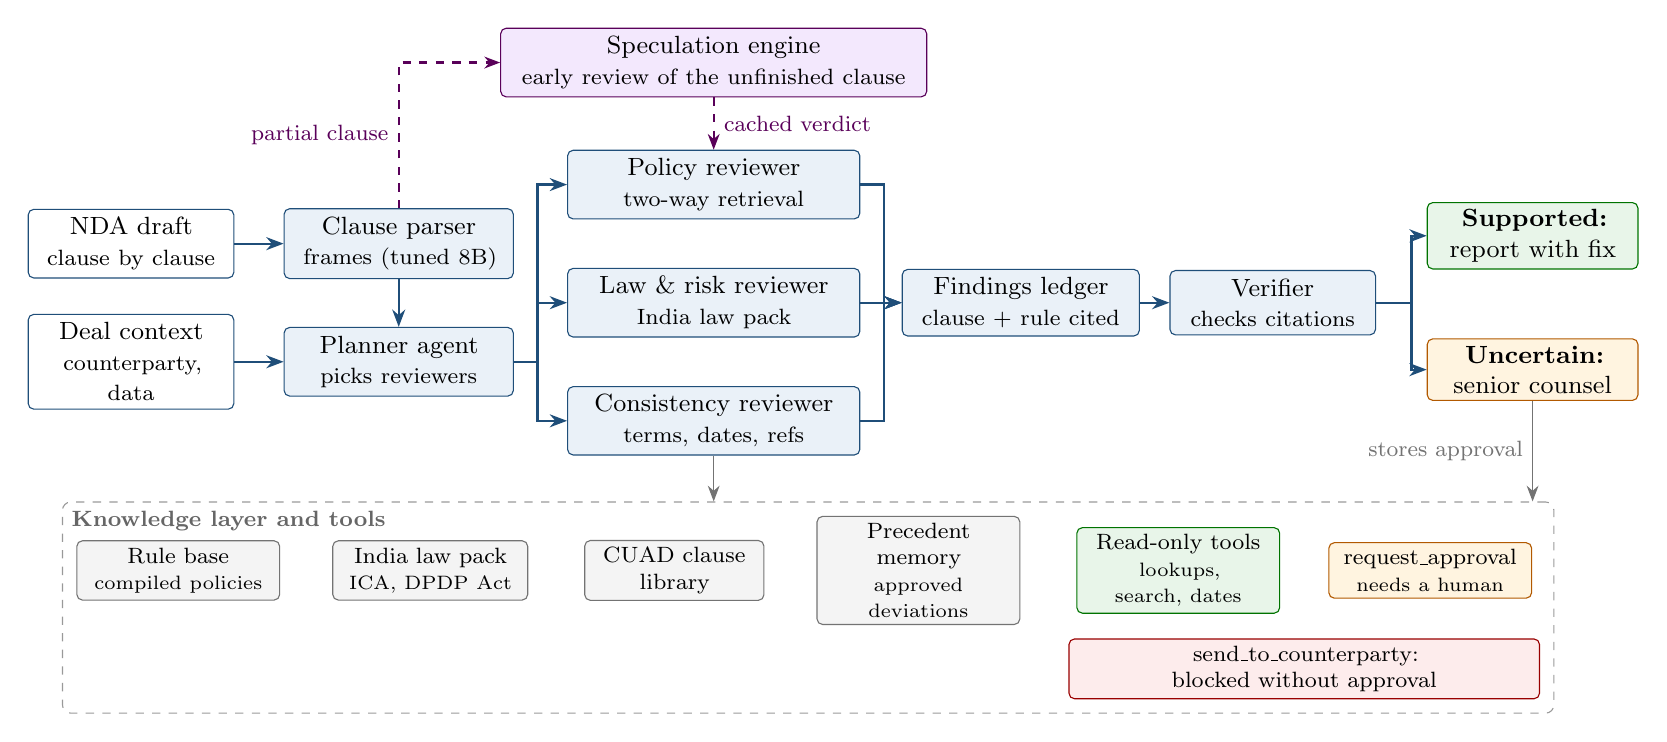
\begin{tikzpicture}
% inputs
\node[box,fill=white,text width=2.4cm] (nda) at (0,0.75) {NDA draft\\\footnotesize clause by clause};
\node[box,fill=white,text width=2.4cm] (ctx) at (0,-0.75) {Deal context\\\footnotesize counterparty, data};
% parser + planner
\node[box,text width=2.7cm] (parse) at (3.4,0.75) {Clause parser\\\footnotesize frames (tuned 8B)};
\node[box,text width=2.7cm] (plan) at (3.4,-0.75) {Planner agent\\\footnotesize picks reviewers};
% reviewers
\node[box,text width=3.5cm] (r1) at (7.4,1.5) {Policy reviewer\\\footnotesize two-way retrieval};
\node[box,text width=3.5cm] (r2) at (7.4,0) {Law \& risk reviewer\\\footnotesize India law pack};
\node[box,text width=3.5cm] (r3) at (7.4,-1.5) {Consistency reviewer\\\footnotesize terms, dates, refs};
% ledger, verifier
\node[box,text width=2.8cm] (led) at (11.3,0) {Findings ledger\\\footnotesize clause + rule cited};
\node[box,text width=2.4cm] (ver) at (14.5,0) {Verifier\\\footnotesize checks citations};
% outputs
\node[ok,text width=2.5cm,font=\small] (rep) at (17.8,0.85) {\textbf{Supported:}\\report with fix};
\node[tool,text width=2.5cm,font=\small] (hum) at (17.8,-0.85) {\textbf{Uncertain:}\\senior counsel};
% speculation
\node[spec,text width=5.2cm] (spec) at (7.4,3.05) {Speculation engine\\\footnotesize early review of the unfinished clause};
% arrows main
\draw[arr] (nda) -- (parse);
\draw[arr] (ctx) -- (plan);
\draw[arr] (parse) -- (plan);
\draw[arr] (plan.east) -- ++(0.3,0) |- (r1.west);
\draw[arr] (plan.east) -- ++(0.3,0) |- (r2.west);
\draw[arr] (plan.east) -- ++(0.3,0) |- (r3.west);
\draw[arr] (r1.east) -- ++(0.3,0) |- (led.west);
\draw[arr] (r2.east) -- (led.west);
\draw[arr] (r3.east) -- ++(0.3,0) |- (led.west);
\draw[arr] (led) -- (ver);
\draw[arr] (ver.east) -- ++(0.45,0) |- (rep.west);
\draw[arr] (ver.east) -- ++(0.45,0) |- (hum.west);
\draw[darr] (parse.north) |- node[pos=0.25,left,font=\footnotesize,violet!70!black]{partial clause} (spec.west);
\draw[darr] (spec.south) -- node[right,font=\footnotesize,violet!70!black]{cached verdict} (r1.north);
% support layer
\node[kb,text width=2.4cm] (kb1) at (0.6,-3.4) {Rule base\\\scriptsize compiled policies};
\node[kb,text width=2.3cm] (kb2) at (3.8,-3.4) {India law pack\\\scriptsize ICA, DPDP Act};
\node[kb,text width=2.1cm] (kb3) at (6.9,-3.4) {CUAD clause\\library};
\node[kb,text width=2.4cm] (kb4) at (10.0,-3.4) {Precedent memory\\\scriptsize approved deviations};
\node[ok,text width=2.4cm] (t1) at (13.3,-3.4) {Read-only tools\\\scriptsize lookups, search, dates};
\node[tool,text width=2.4cm] (t2) at (16.5,-3.4) {request\_approval\\\scriptsize needs a human};
\node[bad,text width=5.8cm] (t3) at (14.9,-4.65) {send\_to\_counterparty: blocked without approval};
\begin{scope}[on background layer]
\node[draw=black!40,dashed,rounded corners=3pt,fit=(kb1)(kb4)(t1)(t2)(t3),inner sep=5pt] (sup) {};
\end{scope}
\node[font=\footnotesize\bfseries,black!60,anchor=north west] at (sup.north west) {Knowledge layer and tools};
\draw[garr] (r3.south) -- (r3.south |- sup.north);
\draw[garr] (hum.south) -- (hum.south |- sup.north) node[pos=0.5,left,font=\footnotesize]{stores approval};
\end{tikzpicture}}
\caption{CounselCopilot architecture. Blue boxes are LLM agents (same backbone in every system we compare). Green tools are read-only and may be called speculatively; orange needs human approval; red is never allowed without approval.}
\end{figure}

\textbf{How it works.} The \emph{clause parser} turns each clause into an \emph{obligation frame} \{party, action, object, condition, duration, exception\}, so numbers and conditions can be compared exactly rather than by text similarity. Offline, a \emph{policy compiler} turns each company's prose policies into a rule base, where every rule has an ID, an applicability condition (e.g.\ \texttt{vendor AND personal\_data}), a requirement and its source text. The \emph{planner} picks reviewers based on the deal and the clause types present. Three reviewers call tools and write findings to a shared ledger. The \emph{verifier} keeps a finding only if both citations (NDA clause and rule or statute) support it, and sends uncertain or approval-gated cases to a senior lawyer. Approved deviations go into \emph{precedent memory}, so the same question is not escalated twice.

\begin{figure}[H]
\centering
\resizebox{0.86\textwidth}{!}{%
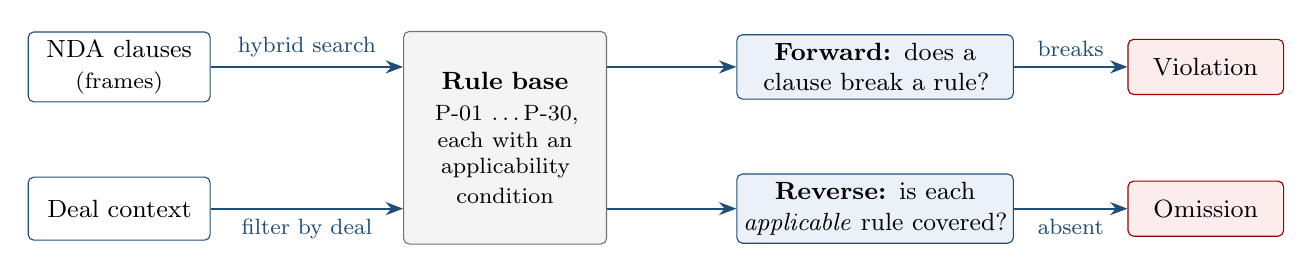
\begin{tikzpicture}
\node[box,fill=white,text width=2.1cm] (cl) at (0,0.9) {NDA clauses\\\footnotesize (frames)};
\node[box,fill=white,text width=2.1cm] (dc) at (0,-0.9) {Deal context};
\node[kb,text width=2.4cm,minimum height=2.7cm,font=\small] (rb) at (4.9,0) {\textbf{Rule base}\\[2pt]\footnotesize P-01 \ldots P-30,\\each with an\\applicability\\condition};
\node[box,text width=3.3cm] (fw) at (9.6,0.9) {\textbf{Forward:} does a clause break a rule?};
\node[box,text width=3.3cm] (rv) at (9.6,-0.9) {\textbf{Reverse:} is each \emph{applicable} rule covered?};
\node[bad,text width=1.8cm,font=\small] (vi) at (13.8,0.9) {Violation};
\node[bad,text width=1.8cm,font=\small] (om) at (13.8,-0.9) {Omission};
\draw[arr] (cl) -- node[above,font=\footnotesize]{hybrid search} (rb.west |- cl);
\draw[arr] (dc) -- node[below,font=\footnotesize]{filter by deal} (rb.west |- dc);
\draw[arr] (rb.east |- fw) -- (fw);
\draw[arr] (rb.east |- rv) -- (rv);
\draw[arr] (fw) -- node[above,font=\footnotesize]{breaks} (vi);
\draw[arr] (rv) -- node[below,font=\footnotesize]{absent} (om);
\end{tikzpicture}}
\caption{Two-way retrieval. The reverse path is the only way to find a \emph{missing} clause, and the deal filter stops rules that don't apply to this deal from firing.}
\end{figure}

\begin{figure}[H]
\centering
\resizebox{0.86\textwidth}{!}{%
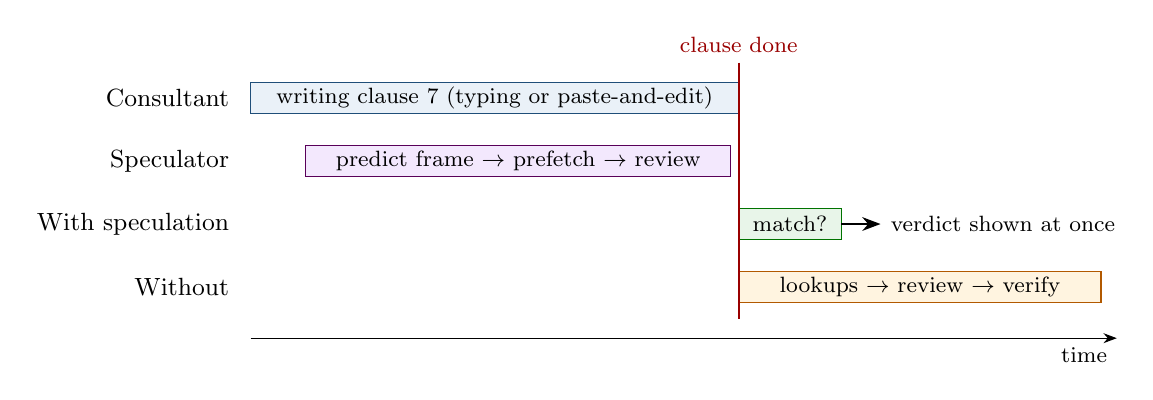
\begin{tikzpicture}[x=1cm,y=1cm]
\node[font=\small,anchor=east] at (-0.15,1.6) {Consultant};
\node[font=\small,anchor=east] at (-0.15,0.8) {Speculator};
\node[font=\small,anchor=east] at (-0.15,0) {With speculation};
\node[font=\small,anchor=east] at (-0.15,-0.8) {Without};
\filldraw[fill=soft,draw=accent] (0,1.4) rectangle (6.2,1.8); \node[font=\footnotesize] at (3.1,1.6) {writing clause 7 (typing or paste-and-edit)};
\filldraw[fill=specc,draw=violet!70!black] (0.7,0.6) rectangle (6.1,1.0); \node[font=\footnotesize] at (3.4,0.8) {predict frame $\rightarrow$ prefetch $\rightarrow$ review};
\filldraw[fill=okc,draw=green!45!black] (6.2,-0.2) rectangle (7.5,0.2); \node[font=\footnotesize] at (6.85,0) {match?};
\filldraw[fill=toolc,draw=orange!70!black] (6.2,-1.0) rectangle (10.8,-0.6); \node[font=\footnotesize] at (8.5,-0.8) {lookups $\rightarrow$ review $\rightarrow$ verify};
\draw[thick,red!60!black] (6.2,2.05) node[above,font=\footnotesize]{clause done} -- (6.2,-1.2);
\draw[-{Stealth},thick] (7.5,0) -- (8.0,0) node[right,font=\footnotesize]{verdict shown at once};
\draw[-{Stealth}] (0,-1.45) -- (11,-1.45) node[below left,font=\footnotesize]{time};
\end{tikzpicture}}
\caption{Speculative clause review. The cached verdict is shown only if the finished clause's frame matches the predicted one on every field the rules test. Otherwise the review runs normally, so the output never changes.}
\end{figure}

\textbf{RAG design.} Retrieval combines BM25 and dense search with a cross-encoder reranker, so legal terms like ``indemnify'' match exactly. Policies are chunked by rule rather than by fixed size, so an exception stays with its rule. A one-hop cross-reference graph pulls in linked approval rules and statutory exceptions. Because Gemini can read a whole 40k-token pack, we do not assume RAG is needed. We \emph{measure} it with a policy-size sweep at 40k, 150k and 400k tokens.

\textbf{Speculation, and its safety boundary.} Only read-only tools and the review computation itself are ever run early. \texttt{request\_approval} and \texttt{send\_to\_counterparty} are never speculated, and a speculative verdict never triggers an action. Speculative RAG (a small drafter writes one finding per evidence source, then the backbone verifies them) is our stretch goal, tested for accuracy.

%================ 5 =================
\section{The five capabilities: why each is needed and how we measure it}
\begin{table}[H]\small
\begin{tabularx}{\textwidth}{@{}p{2.1cm}LL@{}}
\toprule
\textbf{Capability} & \textbf{Why this problem needs it} & \textbf{How we measure it} \\
\midrule
Fine-tuning & One QLoRA Llama-3.1-8B for clause tags (CUAD), ContractNLI checks, obligation frames and drafts. Frames must be exactly structured, and frame prediction runs after every sentence, so it must be local and free. & CUAD tag F1; ContractNLI acc./macro-F1 (12 trained, 5 held-out checks); frame field accuracy on 300 gold frames; tuned vs untuned vs prompted Gemini \\
RAG & An omission check must find \emph{every} applicable rule, cite it exactly and stay cheap as the policy corpus grows. & Applicable-rule recall@k, omission recall, nDCG@10, policy-size sweep vs long context \\
Reasoning & Deciding whether a rule applies to this deal, comparing frames to rules, verifying each finding. & Accuracy of every intermediate applicability decision vs gold; verifier rejection precision; cause of each miss \\
Agentic & Planner, specialist reviewers, shared ledger, precedent memory, hand-off to a senior lawyer. & Planner vs fixed pipeline; hand-off precision/recall; escalations avoided by memory \\
Tool calling & Exact bookkeeping (terms, dates, cross-references), rule/statute/approval lookups, gated actions, prefetching. & Tool precision/recall vs gold tool sets per defect type, argument validity, recovery from 10\% injected errors, \textbf{unsafe action rate (target 0)} \\
\bottomrule
\end{tabularx}
\end{table}

%================ 6 =================
\section{Dataset and evaluation environment: PolicyNDA}
\begin{itemize}
\item \textbf{NDAs:} ContractNLI (607 real NDAs, split 423/61/123, CC BY 4.0). \textbf{Clause library:} CUAD (510 contracts, 41 clause types).
\item \textbf{Company policy packs (we write):} 3 fictional Indian companies, each with $\sim$30 NDA rules buried in $\sim$40k tokens of realistic prose. They are written by teammates who do not build the system, and the gold rule lists are kept separate.
\item \textbf{India law pack:} $\sim$15 clear-cut provisions (ICA s.23/27/28, DPDP Act 2023, Arbitration Act seat rules, Specific Relief Act), each checked by two teammates.
\item \textbf{Ground truth without circularity:} about 60\% of the rules are anchored to ContractNLI's 17 expert-labelled checks (e.g.\ ``vendor NDAs must require return of information'' $\leftrightarrow$ \emph{return of confidential information}). So each real NDA's \emph{natural} omissions and violations are already labelled by legal experts. The remaining field rules (governing law, term length) are hand-labelled by two annotators, with Cohen's $\kappa$ reported.
\item \textbf{Planted defects on top:} violations, omissions, approval-gated deviations, statutory risks, internal inconsistencies, prompt-injection text, and \emph{distractors} (rules that look relevant but don't apply), giving 2--4 per NDA. About 25\% of NDAs get only distractors, so we can measure false alarms.
\item \textbf{Live replay:} each test NDA is replayed as a drafting session in two styles, typed at 40 wpm and paste-a-template-then-edit.
\end{itemize}

%================ 7 =================
\section{Evaluation plan}
\textbf{Two-stage backbone.} Stage 1 runs everything on \textbf{Llama-3.1-8B} served free on Kaggle GPUs. Stage 2 confirms the main systems on \textbf{Gemini 3.8 Flash}. All systems in a comparison use the same backbone. Long-context runs and the policy-size sweep need Gemini, because a T4 GPU cannot hold a 40k-token prompt.

\begin{table}[H]\small
\begin{tabularx}{\textwidth}{@{}>{\raggedright\arraybackslash}p{2.3cm}L@{}}
\toprule
\textbf{Baselines} & B1 long context (whole pack in one prompt) $\cdot$ B2 naive RAG (fixed chunks, forward only) $\cdot$ B3 single agent with tools $\cdot$ B4 exhaustive per-rule checking (PolicyGuard-style) \\
\textbf{Ablations} (one change each) & no reverse retrieval (clean RQ1 test) $\cdot$ no deal filter $\cdot$ no frames $\cdot$ no verifier $\cdot$ planner $\rightarrow$ fixed pipeline $\cdot$ untuned model $\cdot$ no cross-reference graph $\cdot$ no memory $\cdot$ speculation: none / prefetch only / heuristic frames / tuned frames / oracle \\
\textbf{Detection} & Recall, precision and F1 per defect type; \textbf{omission recall}; false alarms per NDA. A finding counts only if both citations are correct. Natural and planted defects are reported separately. \\
\textbf{Speculation} & Time-to-feedback p50/p95 (real measured latency, including GPU contention); reuse rate; agreement of reused verdicts with a full re-run; wasted calls and cost \\
\textbf{Safety} & Unsafe/unapproved action rate (target 0), including prompt-injection text inside NDAs; hand-off precision and recall \\
\textbf{Rigour} & Bootstrap 95\% CIs and McNemar's test. An LLM judge is used only for explanation quality, validated against 100 human labels (Cohen's $\kappa$). Five worked qualitative cases and a table of misses by cause. \\
\bottomrule
\end{tabularx}
\end{table}

%================ 8 =================
\section{Expected novelty}
\begin{enumerate}
\item \textbf{PolicyNDA}, the first \emph{open} benchmark for checking NDAs against company policy. It covers omissions and deal-specific applicability, with ground truth anchored to expert labels.
\item \textbf{Applicability-aware two-way retrieval}, compared honestly against exhaustive per-rule checking and against long context as the policy corpus grows.
\item \textbf{Verified speculative review} for live drafting: reuse is exact rather than approximate, with a strict read-only boundary.
\end{enumerate}

%================ 9 =================
\section{Safety plan}
\begin{itemize}
\item Only public NDAs and synthetic policies, so no client or personal data. Llama runs locally; only public or synthetic text goes to the Gemini API, on the paid tier.
\item Gated actions: \texttt{request\_approval} needs human confirmation, and \texttt{send\_to\_counterparty} is a mock that is blocked without approval. Misuse is measured, including under prompt injection.
\item The output is decision support with citations, not legal advice. No team member is a lawyer, so statutory flags are worded as ``risk under s.27'' and the law pack is small, cited and dated.
\end{itemize}

%================ 10 =================
\section{Compute plan}
\begin{table}[H]\small
\begin{tabularx}{\textwidth}{@{}LXr@{}}
\toprule
\textbf{Item} & \textbf{Resource} & \textbf{Estimate} \\
\midrule
QLoRA Llama-3.1-8B, multi-task, $\sim$18k examples, 2 runs & Kaggle T4 (free) & $\approx$16 GPU-h \\
Tuned-model inference (frames for replay, ContractNLI test) & Kaggle T4, vLLM & $\approx$6 GPU-h \\
Stage 1: all systems and ablations on Llama-8B, 123 NDAs, 2 seeds & Kaggle 2$\times$T4, vLLM & $\approx$30 GPU-h, \$0 \\
Stage 2: B1--B4, full system and 6 core ablations, 123 NDAs ($\approx$68M in / 7M out tokens) & Gemini 3.8 Flash, Batch API & $\approx$\$38 \\
Policy-size sweep, live-latency replay on Gemini & Gemini 3.8 Flash & $\approx$\$35 \\
Silver frames, policy compilation, Pro reference runs & Gemini 3.1 Pro, Batch API & $\approx$\$28 \\
\midrule
\textbf{Total} & & \textbf{$\approx$55 GPU-h, $\approx$\$100} \\
\bottomrule
\end{tabularx}
\end{table}
\vspace{-4pt}
{\small Prices from the official Gemini pricing page (2 Oct 2026): 3.8 Flash costs \$0.75 in / \$3.75 out per million tokens until 31 Dec 2026, then double, so the API total is $\approx$\$175 if stage 2 runs after that date. 55 GPU-hours is about two weeks of Kaggle's free quota.}

%================ 11 =================
\section{Risks and fallback plan}
\begin{table}[H]\small
\begin{tabularx}{\textwidth}{@{}LL@{}}
\toprule
\textbf{Risk} & \textbf{Fallback} \\
\midrule
Scope too large for the time & RQ1 is the core. Speculative RAG is dropped first; speculative review is cheap once frames exist. \\
Long context or exhaustive checking matches our retrieval & Report it. The benchmark, the omission results and the cost difference are still contributions. \\
Llama-8B too weak for tool use & Constrained JSON decoding; move stage 1 to a hosted Llama-70B; run stage 2 regardless. \\
Gains come from memorised ContractNLI labels & 5 checks are held out of fine-tuning and reported separately. \\
Paste-and-edit leaves little time to speculate & Report reuse rate against how much of the clause is written; this is a finding, not a failure. \\
Unrealistic policies or law errors & Model policies on public corporate policies; realism check by a teammate; two-person law check. \\
\bottomrule
\end{tabularx}
\end{table}

\vspace{-4pt}
{\footnotesize\textbf{Key references.} Koreeda \& Manning, ContractNLI (EMNLP Findings 2021) $\cdot$ Hendrycks et al., CUAD (NeurIPS 2021) $\cdot$ CLAUSE (EACL Findings 2026, arXiv:2511.00340) $\cdot$ ContractScrub (arXiv:2608.20204) $\cdot$ ContractEval (NLLP 2025, arXiv:2508.03080) $\cdot$ PolicyGuard (arXiv:2606.32004) $\cdot$ Speculative Interaction Agents (arXiv:2605.13360) $\cdot$ Speculative Actions (ICLR 2026) $\cdot$ Speculative RAG (ICLR 2025) $\cdot$ Lost in the Middle (TACL 2024) $\cdot$ QLoRA (NeurIPS 2023).}

\end{document}
